% =======================
% Chapter: Related Work
%
% Author: Daniel Wehner
%

% -----------------------------------------------------------------------------------------------------------------------------------------------------
% Related Work
\section{Related Work}
\label{sec:rel_work}

\vspace*{-1mm}
% -----------------------------------------------------------------------------------------------------------------------------------------------------
% Chapter Introduction
\subsection{Introduction}
\label{sec:rel_work_intro}

This chapter introduces scientific research which forms the basis for this thesis. Section \vref{sec:rel_work_embeddings} first of all demonstrates which efforts have already been devoted into the creation of monolingual and multilingual word and sentence embedding algorithms. The focus of the subsequent section \vref{sec:rel_work_eval} is on relevant literature involving the evaluation of sentence embeddings. Overall, this chapter is designed to give a general overview of all relevant concepts without explaining them in-depth. If necessary, a more detailed explanation is given in the respective chapters where the concepts are needed.

% -----------------------------------------------------------------------------------------------------------------------------------------------------
% Vectorial Representations of natural Language
\subsection{Vectorial Representations of natural Language}
\label{sec:rel_work_embeddings}

\highlight{Word embeddings.} State-of-the-art \gls{nlp} applications rely on vectorial language representations usually generated by neural networks. The idea to learn representations of natural language -- commonly known as \textbf{embeddings} -- by leveraging such neural architectures is by no means novel. One of the first approaches dates back to the year 2003 when \citep{Bengio.2003} introduced the neural language model which was devised to mitigate the \textbf{curse of dimensionality} when learning the joint probability function of word sequences. This could be achieved \textit{`by learning a \textbf{distributed representation for words}'}. The major breakthrough, however, was achieved approximately ten years later. Back then, \citep{Mikolov.2013a} proposed the famous \textit{word2vec} algorithm which comes in its two well-known flavors, \textit{Skip-Gram} and \textit{\gls{cbow}}. Only one year later, \citep{Le.2014} published another paper containing several extensions to the \textit{Skip-Gram} model. Two methods, namely \textbf{negative sampling} and \textbf{sub-sampling of frequent words} were developed to increase the robustness of the resulting word embeddings.

In the following years, many were to join this line of research and new approaches to embedding natural language were invented. Among them is a word  embedding called \textit{GloVe} proposed by \citep{Pennington.2014}. In contrast to \textit{word2vec}, this algorithm also takes \textbf{global corpus statistics} into account to improve the representations learned. Another example is \textit{FastText}, an algorithm which includes \textbf{sub-word information} by averaging character $n$-grams \citep{Bojanowski.2017}. This model is perfectly suited to handle \gls{oov} words. \citep{Mrksic.2017} further propose to fine-tune word embeddings by leveraging \textbf{linguistic constraints} like synonymy/antonymy relationships. This idea gives rise to an algorithm called \textit{Attract-Repel}. More recently, \textbf{contextualized word embeddings} have emerged. Examples include \textit{\gls{bert}} \citep{Devlin.2018} which builds on the transformer architecture \citep{Vaswani.2017} and \textit{\gls{elmo}} \citep{Peters.2018}. Such embeddings assign word representations based on the surrounding words. This way it is possible to model \textbf{polysemous words}, i.\,e. words that can have different meanings in different contexts.

\highlight{Sentence embeddings.} Soon the question arose whether it is feasible to embed even larger spans of text that go beyond single words. The notion of sentence embeddings was born. \citep{Yang.2018} differentiate between \textbf{non-parametric} and \textbf{parametric} algorithms, where techniques of the first kind (a.\,k.\,a. compositional models) are quite frequently applied and often serve as a baseline for more elaborate ones. In this context, each word in the sentence is represented by a word embedding produced by a freely-selectable word embedding algorithm which maps words to vectors. These word embeddings subsequently undergo a pooling procedure to obtain a single sentence representation. Many different pooling strategies have already been investigated in the literature: These range from average-, min-, or max-pooling to more sophisticated strategies like \textit{hierarchical pooling}. \citep{Shen.2018} named these kind of pooling algorithms \textit{\glspl{swem}}. Further, \citep{Rueckle.2018} suggest to concatenate various power means to improve the expressiveness of sentence embeddings. Other approaches like \textit{\gls{sif}} \citep{Arora.2017} or \textit{\gls{gem}} \citep{Yang.2018} make use of a method called \gls{svd}/\gls{pca} to remove projections on principal components before averaging.

Parametric methods, on the other hand, \textbf{train sentence embeddings from scratch}. One of the examples can be regarded as a generalization of the \textit{Skip-Gram} model to the sentence level. Its inventors called the algorithm \textit{Skip-Thought} \citep{Kiros.2015}. \citep{Logeswaran.2018} reformulate \textit{Skip-Thought}'s objective as a multi-class prediction problem to address several issues of the original model. Other algorithms include \textit{InferSent} \citep{Conneau.2017} which is trained on the \textit{\gls{snli}} data set \citep{Bowman.2015} and \textit{sent2vec} \citep{Pagliardini.2018} which computes sentence embeddings by averaging character $n$-grams like \textit{FastText}, but on sentence level. Recently, \citep{Reimers.2019} have introduced \	\textit{\gls{sbert}}, a version of \gls{bert} which is designed to create sentence embeddings.

\highlight{Multi-lingual embeddings.} Next to monolingual embeddings, it is also possible to train multilingual representations, i.\,e. embeddings for more than one language that share an embedding space. One of the first approaches was proposed by \citep{Chandar.2013} who trained bi-lingual auto-encoders. \citep{Espana-Bonet.2017} leverage \gls{mt} architectures to create bilingual embeddings while \citep{Zhou.2016} try to align the representations of documents and their translated counterparts by minimizing the Euclidean distance between the two. More recently, \citep{Artetxe.2018} introduce \textit{massively multilingual sentence embeddings} which are integrated into the \textit{\gls{laser}} library.\footnote{In the following, these embeddings will be referred to as \textit{LASER} embeddings.}\footnote{Cf. \url{https://github.com/facebookresearch/LASER} (retrieved: September 04, 2019)} The model is trained in a multi-lingual fashion and all languages share a joint embedding space. Thus, the same model can be used for a variety of languages. Currently, 93 languages are supported. \textit{\gls{bert}}, too, offers a multilingual version which can be used to obtain embeddings in 104 different languages.\footnote{\url{https://github.com/google-research/bert/blob/master/multilingual.md} (retrieved: September 04, 2019)}

% -----------------------------------------------------------------------------------------------------------------------------------------------------
% Evaluation of Word and Sentence Embeddings
\subsection{Evaluation of Word and Sentence Embeddings}
\label{sec:rel_work_eval}

While sentence embeddings are nowadays well-established in the \gls{nlp} community, it is not entirely clear what features of sentences these embeddings encode \citep[inter alia]{Conneau.2018a}. Sentence representations are \textbf{far from being universal} \citep{Perone.2018}, i.\,e. there is no embedding that fits perfectly to all tasks. The knowledge about which linguistic properties of a sentence are learned by individual sentence embedding algorithms is therefore crucial for the choice of the best technique for the problem at hand.

A classical approach frequently applied to evaluate sentence representations is to use them in downstream applications. In such a setting, the quality of the embeddings can be judged with respect to their performance in a real-word scenario. Naturally, this provides useful insights. However, \citep{Conneau.2018a} point out that \textbf{such evaluations are encoder-specific and results obtained in one setting are not necessarily predictive of the performance in another setting}. In order to mitigate this shortcoming, they introduced a set of ten so-called \textit{probing tasks} which they define to be \textbf{\textit{`classification problem[s] that [focus] on simple linguistic properties of sentences'}}. According to the authors, probing tasks have the following advantages over downstream applications:

\begin{enumerate}[label=\color{tud9c}\textbf{\theenumi.}]
	\item Probing tasks are accompanied by \textbf{easier interpretability} due to their simplicity.
	\item It is less difficult to \textbf{control for biases}. For example \citep{Lai.2014} could show that a
 		classifier can achieve high accuracy scores on the \textit{SICK-E} data set \citep{Marelli.2014} by
 		focusing on explicit negation words. With less complex probing tasks it is much easier to detect such hidden biases and idiosyncrasies
 		of the data set which the model exploits.
	\item The concept of probing tasks is \textbf{independent of the encoder architecture}. All previously introduced
	 	evaluation methods were designed for specific use cases like e.\,g. \gls{mt}. As a consequence, it was not straightforward to
 		transfer them to other settings or embedding architectures.
\end{enumerate}

\citep{Conneau.2018a} categorized the tasks into three distinct types: \ding{182} \textbf{Surface information tasks}, \ding{183} \textbf{syntactic tasks} as well as \ding{184} \textbf{semantic tasks}. The authors designed all the probing tasks to fulfill the following requirements:

\begin{enumerate}[label=\color{tud9c}\textbf{\theenumi.}]
	\item A probing task only takes \textbf{single sentence representations as input}. This also excludes feeding additional input
	 	like word embeddings into the classifier. This would severely affect the evaluation results in a negative way, since the
 		performance cannot be traced back clearly to the sentence representation alone.
	\item The probing tasks setup should allow for the creation of
		\textbf{large training and validation sets}. According to \citep{Conneau.2018a}, large amounts of data may be necessary,
		 since the linguistic information might be encoded in a non-linear fashion. Non-linear classifiers are usually characterized
		 by a vast amount of parameters which require more data to be tuned properly.
	\item It should be possible to \textbf{control for `nuisance factors' and `hidden biases'}.
	\item The tasks should \textbf{`cover an interesting set of linguistic properties'}.
\end{enumerate}

The work of \citep{Conneau.2018a} was inspired by pioneering efforts made by \citep{Ettinger.2016,Shi.2016,Adi.2017} who were the first to introduce the notion of probing tasks. \citep{Shi.2016} were primarily interested in the question whether \gls{mt} systems can learn source syntax. In this context they proposed so-called \textbf{syntactic labels} to probe sentences for syntactical properties. \citep{Adi.2017}, on the other hand, put the focus on testing embeddings for surface information (e.\,g. the length of a sentence or the  containment of words, etc.). \citep{Ettinger.2016} were above all interested in semantic information retained by sentence embeddings. He and his colleagues introduced tasks which make use of \textbf{semantic roles} and probed sentences for \textbf{entity-event relationships}. Further probing tasks and evaluation methodologies were introduced by \citep{Zhu.2018} who made use of cosine similarities to evaluate sentence embeddings. They constructed triplets of sentences $S$, $S^*$ and $S^+$ by having the original sentences undergo \textbf{sentence modification schemes} like \textit{`passivization'}, \textit{`synonym substitution'} or \textit{`quantifier negation'}. For instance, they constructed a sentence triplet: ($S$: \textit{`The fox is jumping over the dog'}, $S^*$: \textit{`The fox is not jumping over the dog'}, $S^+$: \textit{`The fox is hopping over the sleeping dog'}). Despite the fact that sentences $S$ and $S^*$ exhibit a quite similar surface form, their meaning is antonymous. On the other hand, $S$ and $S^+$ use quite different words but have a similar meaning. Hence, \citep{Zhu.2018} claim that the similarity of $S$ and $S^*$ should be smaller than the one between $S$ and $S^+$: $\text{sim}(S, S^*) < \text{sim}(S, S^+)$. Embeddings complying with this requirement will get a positive test result.

\citep{Linzen.2016,Gulordava.2018} probed \gls{rnn} representations for long-range dependencies such as subject-verb relations and mainly found that such representations fail to properly represent long-range dependencies. \citep{Naik.2018} created so-called \textbf{stress test data sets} to investigate errors of \gls{nli} classifiers. The authors found that if premise and hypothesis sentences have a large word overlap, the model is often inclined to label the sentence pair as an entailment, even if the sentences have no common meaning. If the overlap is small, related sentences are often labeled as neutral. Based on this error analysis, large-scale data sets were constructed aiming at testing models for such phenomena. The authors distinguish between \textbf{competence tests}, \textbf{distraction tests} and \textbf{noise tests}. If the model wants to excel at competence tests, it has to perform complex reasoning. Distraction test data sets contain adversarial examples which aim to elicit a false prediction from the model whereas noise tests give insight into whether the model is robust with respect to spelling errors.

\textbf{The evaluation of vectorial representations of sentences is often restricted to the English language and only a small number of researchers also consider a multilingual setting.} \citep{Cer.2017} for example published semantic similarity data sets in four languages dedicated to evaluation. Other authors released multilingual training and evaluation data which were either produced by translating English resources \citep{Agic.2017,Mehdad.2011} or by additional annotation of parallel corpora \citep{Negri.2011}. \citep{Conneau.2018c} created a new English data set similar to the MuliNLI data set \citep{Williams.2018}, but translated it into 15 languages, including some low-resource languages like Urdu. \citep{Sahin.2019} use multilingual probing tasks for word embeddings in  several languages. They point out that English is rather poor from a morphological point of view and that different results have to be expected in other languages which are more diverse. In fact, they found that correlations between probing and downstream task results tend to be higher in morphologically richer languages. Very recently, \citep{Krasnowska.2019} have extended on the ideas of Conneau and colleagues by introducing a slightly modified set of probing tasks for the Polish language. They further enriched Conneau's suite of probing tests with the \caps{Passive} task which probes for voice information. They mainly found that \textit{LASER} embeddings can be considered superior to other techniques, yet they were unable to give specific reasons for the outstanding performance of this sentence encoder.

\citep{Ravishankar.2019} conduct an evaluation on five different languages (English, French, German, Spanish and Russian) using the set of Conneau's probing tasks with minor modifications. The encoder architecture the authors leverage is very similar to the one used for the \textit{InferSent} model (cf. section \vref{sec:infersent}). The encoder also uses \textit{FastText} word embeddings as a basis.

\ding{182} As a first step, the authors map the \textit{FastText} embeddings for all languages into the English embedding space using the \textit{VecMap} approach introduced by \citep{Artetxe.2016}. \ding{183} Subsequently, they train an English encoder (cf. left-hand side of figure \vref{fig:x_probe}) on high-quality \gls{nli} data. \ding{184} In the next phase, the authors encode parallel sentences, where the first sentence is given in English and the second one is its translated counterpart in one of the target languages. The English sentence is encoded using the trained English encoder from before (cf. step \ding{183}), whereas the target-language sentence is encoded using a different encoder whose weights are initialized randomly. This encoder is subsequently trained on the mean squared error between its output and the English representation (this step is illustrated in the middle part of figure \vref{fig:x_probe}). This procedure is repeated for all languages. \ding{185} After training, the target-language encoder is used in the probing tasks as usual (cf. right-hand side of figure \vref{fig:x_probe}). The evaluation on probing tasks is then conducted on parallel data the authors extracted from Wikipedia. The encoder mapping procedure was first introduced by \citep{Conneau.2018c}.

% Figure: Multilingual mapping of encoders
\begin{figure}[h]
	\centering
	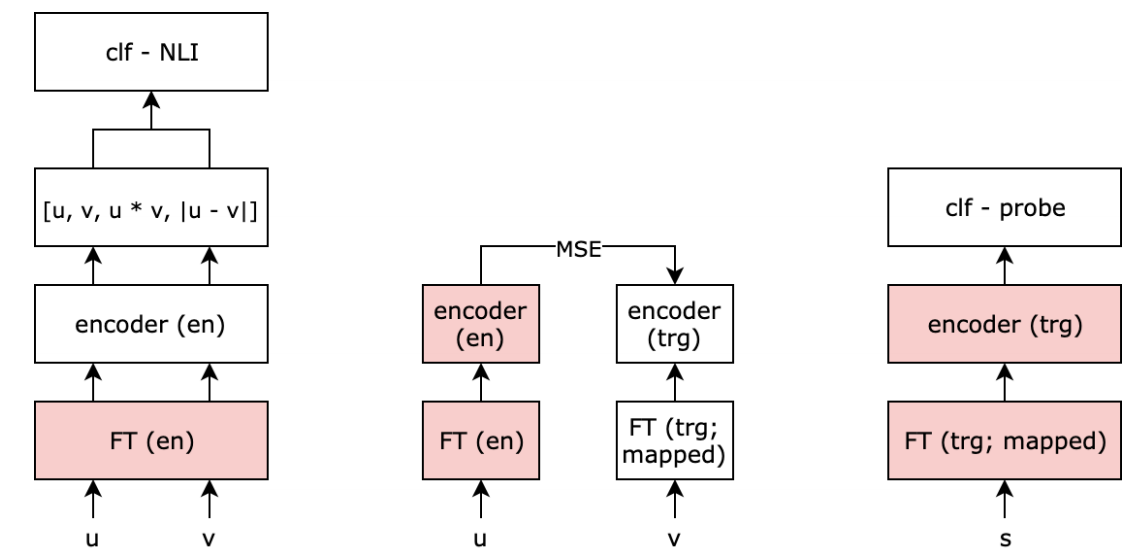
\includegraphics[scale=0.35]{images/x_probe}
	\caption[Encoder mapping procedure employed by Ravishankar and colleagues]
		{Illustration of the encoder mapping procedure employed by \citep{Ravishankar.2019}.
		The image was taken from \citep{Ravishankar.2019}}
	\label{fig:x_probe}
\end{figure}

\citep{Conneau.2018b} furthermore noticed that there was \textbf{no standard approach to the evaluation of sentence embeddings}. In each publication, different setups were used such that comparisons between individual results started to lack validity. As a consequence, they developed the \textit{SentEval} framework, an easy-to-use open-source Python project\footnote{\url{https://github.com/facebookresearch/SentEval} (retrieved: September 03, 2019)} which comes with diverse downstream classification tasks as well as the set of probing tasks introduced by \citep{Conneau.2018a}. \citep{Perone.2018} made use of this framework to conduct a comprehensive study in which they evaluated more state-of-the-art embedding architectures. Their experiments confirmed that there is no universal sentence embedding and furthermore showed that a \gls{bov} approach using contextualized \textit{ELMo} embeddings achieves high performance across many probing tasks.

Despite the convenient usage of such frameworks, \citep{Eger.2019} still notice several pitfalls that many researchers frequently tab into when it comes to probing sentence representations. These pitfalls include e.\,g. \textbf{using different classifier architectures} for the evaluation or \textbf{comparing sentence embeddings of different sizes}. The latter issue was already realized by \citep{Rueckle.2018} who pointed out that comparing usually low-dimensional average methods to higher-dimensional trained embeddings was unfair and therefore proposed to concatenate several average embeddings to increase their dimensionality. Finally, in order to facilitate a better evaluation, \citep{Eger.2019} conjecture that the set of downstream applications should be enriched with more demanding tasks where simple compositional models and random encoders are outperformed by trained encoder architectures more decisively.

\begin{tudbox}{Motivation and Goal of this Thesis}
\textbf{The above explanations show that the number of researchers taking a multi-lingual setting into account is small but increasing steadily. Nevertheless, the set of languages is still often limited to high-resource languages like German, French or Spanish. Overall, much less research could be found that focuses on probing sentence embeddings in lower-resource languages. It is therefore unclear whether the results obtained for high-resource languages are generalizable to languages for which by far less data is available. This circumstance makes it worthwhile to put lower-resource languages more in focus. Providing more insight into sentence embeddings in lower-resource languages is the goal of this thesis.}
\end{tudbox}

% -----------------------------------------------------------------------------------------------------------------------------------------------------
% Chapter Summary
\subsection{Summary}
\label{sec:rel_work_summary}

This chapter introduced the foundational work for this thesis. The literature review made clear that a large number of sentence embedding algorithms exists. However, large-scale evaluations of these techniques have long been neglected. What is more, before the release of \textit{SentEval}, no standard framework existed which could be used to assess the quality of the embeddings in a comparable way. Also, the probing task literature is mostly restricted to the English language, but successively, more and more researches are beginning to shift their focus to other languages which are morphologically richer than English. Most of the time only high-resource languages are taken into account, while low-resource languages are omitted. \textbf{This is why the present thesis aims to extend the probing task methodology to lower-resource languages in order to investigate whether the patterns found for high-resource languages are still reproducible if by far less resources are available.}
